\chapter{Postestimation}\label{ch:postest}

\section{Goodness of fit: estat gof}\label{sec:gof}

\texttt{estat gof} simulates \opt{nsim()} outcome vectors (default 1000) from the fitted model and compares the statistics of the simulated vectors with the observed ones. For each statistic it reports the observed value, the mean and the standard deviation of the simulated values, and the t-ratio $(\text{simulated mean}-\text{observed})/\text{simulated standard deviation}$; the last line is the Mahalanobis distance of the observed statistics from the simulated ones (with the pseudo-inverse of the covariance matrix if it is singular). The statistics of the model come first: after a converged fit their t-ratios are near 0. Then come statistics that are not in the model (\opt{extra(list)}: any effects; the default, as in \alaamee{}, is the two-stars, three-stars, partner-activity two-paths, triangles, the indirect-partner and the partner-partner effects for undirected networks, and the sender, receiver, reciprocity, star, mixed-star, contagion and triangle effects for directed ones; \opt{noextra} gives none). A t-ratio beyond 0.3 in absolute value is marked. \texttt{r(gof)} holds the table (observed, simulated mean, standard deviation, t-ratio) and \texttt{r(mahalanobis)} the distance. Two plots are available, described in Section~\ref{sec:plots}.

The Lazega fit fits well on the statistics that are not in the model:
\showlog{lazega_diag}
and the Glasgow model fits less well on a few of the extra statistics (the marked rows), which is a hint that the model lacks an effect, for example one for the two-stars between actors with the outcome:
\showlog{glasgow_gof}
The simulation starts from the observed outcomes; \alaamee{} starts from random outcomes. The burn-in is meant to remove the dependence on the start.

\paragraph{When the distribution has two modes.} The simulation can be misleading when the distribution of the outcome has two modes, all or none of the actors with the outcome, which is a common near-degeneracy of contagion models on small networks: the simulated mean statistics lie between the modes and no t-ratio is small. The karate club is an example; the t-ratios of all statistics, including those in the model, are about $0.4$ although the estimate equals the exact maximum likelihood estimate:
\showlog{karate_gof}
Read such a table as a sign of two modes, not as lack of fit.

\section{Convergence: estat mcmcdiag}

\texttt{estat mcmcdiag} reports the convergence diagnostics of the fit. After \opt{method(sa)}: the estimate, the convergence statistic of each coefficient in the final phase (below $0.1$ in absolute value is converged) and the autocorrelation of the simulated differences. After \opt{method(ee)}: for each coefficient the mean and the standard deviation over the runs, the mean and the maximum convergence statistic, the number of runs beyond \opt{threshold()} and the lag-1 autocorrelation of the thinned values of the coefficient and of the differences. \opt{plot} draws the trace of the first EE run (coefficients and differences against the iteration) or the differences of the final phase of the stochastic approximation (Section~\ref{sec:plots}). It is not available after \opt{mple} (r(498)). Examples are in Sections~\ref{sec:first} and~\ref{sec:ee}.

\section{Plots}\label{sec:plots}

Two plots belong to \texttt{estat gof} and one to \texttt{estat mcmcdiag}. They need the \texttt{nwcommands} core 3.29.0 or later (with an older core the plot stops with return code 199 and a message); the commands without a plot do not need it.

\paragraph{Goodness of fit: t-ratios.} \opt{plot} draws the t-ratios of the table as a bar plot, the statistics of the model in one colour and the other statistics in another. The figure shows it for the karate club, after the fit of Section~\ref{sec:first} (the \opt{title("")} option removes the default title):
\begin{lstlisting}
. estat gof, nsim(1000) seed(7) plot title("") export(fig_gof.pdf)
\end{lstlisting}
\begin{figure}[ht]\centering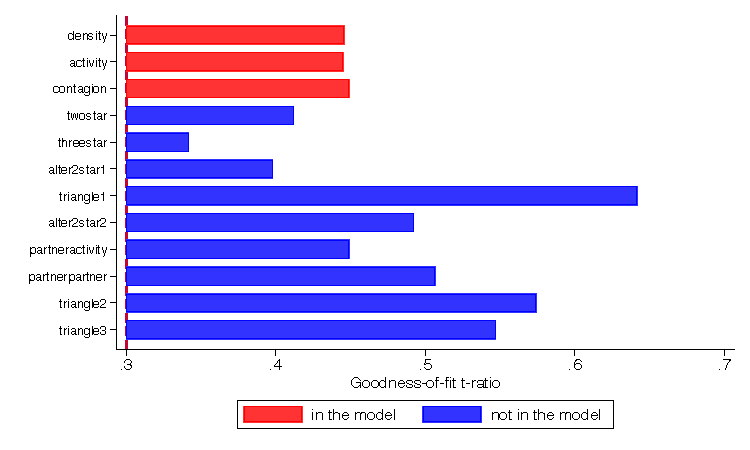
\includegraphics[width=0.75\textwidth]{fig/fig_gof.pdf}
\caption{\texttt{estat gof, plot} after the karate-club fit: t-ratios (all near $0.4$ because the distribution has two modes, see above).}\end{figure}

\paragraph{Goodness of fit: distributions.} \opt{distplot} draws, for every statistic of the model, the histogram of the simulated values with the observed value as a red line; \opt{all} adds the other statistics of the table. It shows what a t-ratio hides: whether the observed value lies in the bulk of the simulated distribution, in its tail, or between two modes. This picture is an extension; \alaamee{} reports the t-ratios only.
\begin{lstlisting}
. estat gof, nsim(1000) seed(7) distplot export(fig_gofdist.pdf)
\end{lstlisting}
\begin{figure}[ht]\centering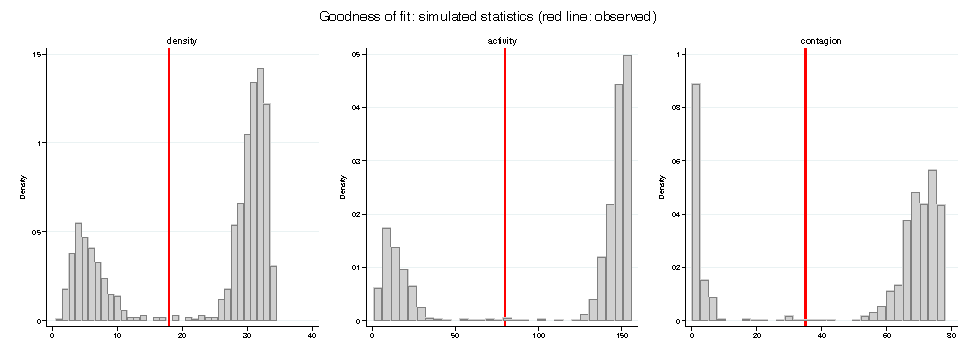
\includegraphics[width=\textwidth]{fig/fig_gofdist.pdf}
\caption{\texttt{estat gof, distplot} for the karate club. The simulated values pile up near none and near all of the actors having the outcome (two modes); the observed values (red lines) lie between the modes, which is why all t-ratios are about $0.4$ although the estimate is the maximum likelihood estimate.}\end{figure}

\paragraph{Convergence: traces.} After an equilibrium-expectation fit, \texttt{estat mcmcdiag, plot} draws the trace of the first run, with the coefficient in the left panel of each effect and the difference between the simulated and the observed statistic (\texttt{dzA}) in the right panel, against the iteration; the vertical dashed line marks the end of the burn-in. A coefficient that still drifts at the end of the run (the density coefficient in the figure) is a sign that more iterations are needed. After stochastic approximation the plot shows the differences of the final phase.
\begin{lstlisting}
. nwalaam faction karate, effects(density activity contagion) method(ee) seed(20261118)
. estat mcmcdiag, plot title("") export(fig_trace.pdf)
\end{lstlisting}
\begin{figure}[ht]\centering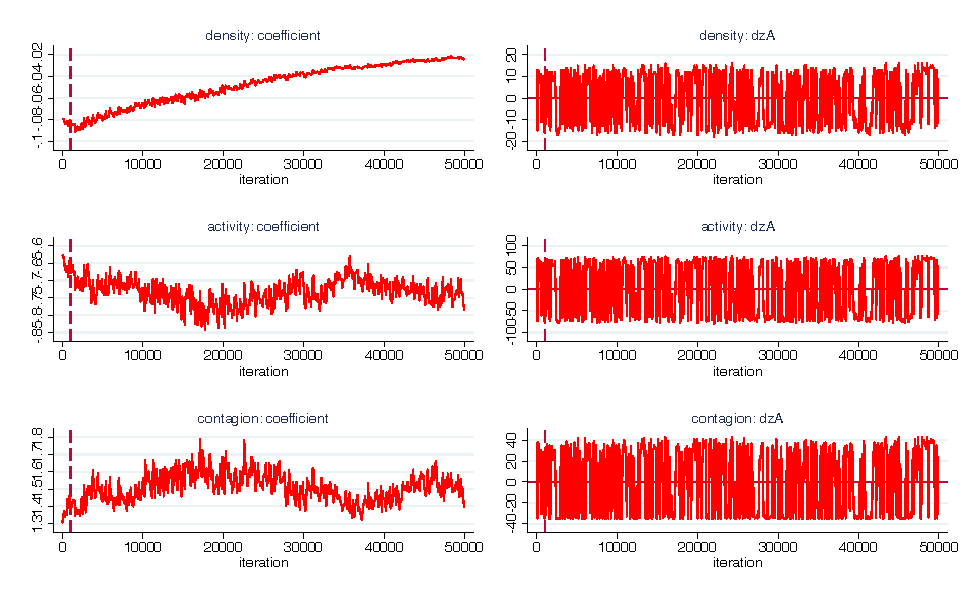
\includegraphics[width=\textwidth]{fig/fig_trace.pdf}
\caption{\texttt{estat mcmcdiag, plot} after \opt{method(ee)} on the karate club: trace of the first run.}\end{figure}

\paragraph{Names, saving and graph options.} The plots follow one convention. \opt{name(name)} names the graph in memory; the defaults are \texttt{nwalaam\_gof} (\opt{plot}), \texttt{nwalaam\_gofdist} (\opt{distplot}) and \texttt{nwalaam\_trace} (\texttt{estat mcmcdiag}). \opt{saving(filename)} saves the graph as a \texttt{.gph} file, and \opt{export(filename)} exports it with \texttt{graph export}, the extension of the file name (\texttt{.pdf}, \texttt{.png}, \dots) setting the format; options of \texttt{graph export} may follow after a comma, as in \opt{export(fig.png, width(1600))}. \opt{saving()} and \opt{name()} accept a trailing \opt{, replace}. Any other graph option is passed on to \texttt{twoway} (\opt{plot}) or to \texttt{graph combine} (\opt{distplot} and the trace plot), for example \opt{title()}, \opt{xsize()} or \opt{scheme()}; the titles of the plots are black, and \opt{title()} replaces the default title. \opt{name()}, \opt{saving()}, \opt{export()} or a graph option without \opt{plot} (or \opt{distplot}) is an error (return code 198):
\showlog{plots_err}

\section{Simulation: nwalaam simulate}\label{sec:simulate}

\texttt{nwalaam simulate} draws outcome vectors from the model with the toggle sampler, the sampler of the estimation. After a fit, with no further arguments, it uses the fitted model and its coefficients; otherwise it needs \emph{outcome}, \emph{network}, \opt{effects()} and the coefficients \opt{theta()} (a $1\times P$ matrix). \opt{generate(stub)} writes the draws to the variables \emph{stub}1, \emph{stub}2, \dots (one row per actor, like the outcome; \opt{replace} overwrites), \opt{frame(name)} to a frame with the variable \texttt{actor} and one variable \texttt{sim}$j$ per draw. The chain starts at the observed outcome; \opt{burnin()} proposals (default the larger of 10,000 and 100 times the number of actors) precede the first draw and \opt{interval()} proposals (default the larger of 1,000 and 10 times the number of actors) lie between draws. Missing outcomes stay missing; the same \opt{seed()} gives the same draws. \opt{mode()}, \opt{zone()} and \opt{sampler()} are as in the fit. The simulation returns in \texttt{r()} the number of draws, the seed, the burn-in, the interval and the observed statistics.
\showlog{lazega_sim}
The 200 draws have about 39 actors with the outcome, the observed number is 41.

\section{Stored results}\label{sec:results}

\begin{longtable}{@{}p{0.3\textwidth}p{0.66\textwidth}@{}}
\toprule Result & Content \\ \midrule \endhead
\multicolumn{2}{@{}l}{\textbf{Matrices}} \\
\texttt{e(b)}, \texttt{e(V)} & The coefficients and their covariance matrix. \\
\texttt{e(obs\_stats)} & The observed statistics. \\
\texttt{e(b\_mple)} & The pseudo-likelihood estimate (missing when it does not exist). \\
\texttt{e(b\_start)} & The starting values. \\
\texttt{e(tratio)}, \texttt{e(diag)} & The convergence statistics and the diagnostics. \\
\texttt{e(run\_diag)}, \texttt{e(trace1)} & Per-run diagnostics, and the trace of the first run (equilibrium expectation). \\
\multicolumn{2}{@{}l}{\textbf{Scalars}} \\
\texttt{e(N)}, \texttt{e(n\_ones)}, \texttt{e(nodes)} & Actors with a non-missing outcome, with the outcome, and nodes of the network (both levels in a two-mode network). \\
\texttt{e(runs)}, \texttt{e(runs\_used)}, \texttt{e(iterations)}, \texttt{e(thin)}, \texttt{e(burnin)}, \texttt{e(proposals)}, \texttt{e(acceptance)}, \texttt{e(seed)} & Equilibrium expectation: the settings, the runs used and the acceptance rate. \\
\texttt{e(repetitions)}, \texttt{e(sa\_converged)}, \texttt{e(saiter)} & Stochastic approximation: the repetitions made, whether the criterion was reached, and the iterations per phase. \\
\multicolumn{2}{@{}l}{\textbf{Macros}} \\
\texttt{e(cmd)}, \texttt{e(version)}, \texttt{e(title)} & \texttt{nwalaam}, the version, the title. \\
\texttt{e(depvar)}, \texttt{e(network)}, \texttt{e(effects)}, \texttt{e(effects\_spec)} & The outcome, the network, the names of the effects and the effects as specified. \\
\texttt{e(method)} & \texttt{sa}, \texttt{ee} or \texttt{mple}. \\
\texttt{e(directed)}, \texttt{e(twomode)}, \texttt{e(modeopt)}, \texttt{e(zone)}, \texttt{e(sampler)} & Properties of the data and the sampler. \\
\bottomrule
\end{longtable}
